\documentclass[a4,useAMS,usenatbib,usegraphicx]{latex/mn2e} 
%\documentclass{latex/emulateapj} 
%External Packages and personalized macros
%=========================================================================
%		EXTERNAL PACKAGES
%=========================================================================
\usepackage{amsmath} 
\usepackage{amssymb} 
\usepackage[section]{placeins}
\usepackage {graphicx}
%\usepackage{graphics}
\usepackage[dvips]{epsfig}
\usepackage{epsfig}  
\usepackage{color}
\usepackage[normalem]{ulem}
\usepackage{hyperref}
\usepackage{caption}
%Non reposionated tables
\usepackage{float}
\restylefloat{table}

%=========================================================================
%		INTERNAL MACROS
%=========================================================================
\def\be{\begin{equation}}
\def\ee{\end{equation}}
\def\ba{\begin{eqnarray}}
\def\ea{\end{eqnarray}}

% To highlight comments 
\definecolor{red}{rgb}{1,0.0,0.0}
\newcommand{\red}{\color{red}}
\definecolor{darkgreen}{rgb}{0.0,0.5,0.0}
\newcommand{\SRK}[1]{\textcolor{darkgreen}{\bf SRK: \textit{#1}}}
\newcommand{\SRKED}[1]{\textcolor{darkgreen}{\bf #1}}

\newcommand{\LCDM}{$\Lambda$CDM~}
\newcommand{\beq}{\begin{eqnarray}}  
\newcommand{\eeq}{\end{eqnarray}}  
\newcommand{\zz}{$z\sim 3$} 
\newcommand{\apj}{ApJ}  
\newcommand{\apjs}{ApJS}  
\newcommand{\apjl}{ApJL}  
\newcommand{\aj}{AJ}  
\newcommand{\mnras}{MNRAS}  
\newcommand{\mnrassub}{MNRAS accepted}  
\newcommand{\aap}{A\&A}  
\newcommand{\aaps}{A\&AS}  
\newcommand{\araa}{ARA\&A}  
\newcommand{\nat}{Nature}  
\newcommand{\physrep}{PhR}
\newcommand{\pasp}{PASP}    
\newcommand{\pasj}{PASJ}    
\newcommand{\avg}[1]{\langle{#1}\rangle}  
\newcommand{\ly}{{\ifmmode{{\rm Ly}\alpha}\else{Ly$\alpha$}\fi}}
\newcommand{\hMpc}{{\ifmmode{h^{-1}{\rm Mpc}}\else{$h^{-1}$Mpc }\fi}}  
\newcommand{\hGpc}{{\ifmmode{h^{-1}{\rm Gpc}}\else{$h^{-1}$Gpc }\fi}}  
\newcommand{\hmpc}{{\ifmmode{h^{-1}{\rm Mpc}}\else{$h^{-1}$Mpc }\fi}}  
\newcommand{\hkpc}{{\ifmmode{h^{-1}{\rm kpc}}\else{$h^{-1}$kpc }\fi}}  
\newcommand{\hMsun}{{\ifmmode{h^{-1}{\rm {M_{\odot}}}}\else{$h^{-1}{\rm{M_{\odot}}}$}\fi}}  
\newcommand{\hmsun}{{\ifmmode{h^{-1}{\rm {M_{\odot}}}}\else{$h^{-1}{\rm{M_{\odot}}}$}\fi}}  
\newcommand{\Msun}{{\ifmmode{{\rm {M_{\odot}}}}\else{${\rm{M_{\odot}}}$}\fi}}  
\newcommand{\msun}{{\ifmmode{{\rm {M_{\odot}}}}\else{${\rm{M_{\odot}}}$}\fi}}  
\newcommand{\lya}{{Lyman$\alpha$~}}
\newcommand{\clara}{{\texttt{CLARA}}~}
\newcommand{\rand}{{\ifmmode{{\mathcal{R}}}\else{${\mathcal{R}}$ }\fi}}  
%SAMPLES
\newcommand{\GHBDM}{\texttt{GH}$_{\mbox{\tiny{BDM}}}$ }
\newcommand{\GHFOF}{\texttt{GH}$_{\mbox{\tiny{FOF}}}$ }
\newcommand{\IHBDM}{\texttt{IH}$_{\mbox{\tiny{BDM}}}$ }
\newcommand{\IHFOF}{\texttt{IH}$_{\mbox{\tiny{FOF}}}$ }
\newcommand{\PBDM}{\texttt{P}$_{\mbox{\tiny{BDM}}}$ }
\newcommand{\PFOF}{\texttt{P}$_{\mbox{\tiny{FOF}}}$ }
\newcommand{\IPBDM}{\texttt{IP}$_{\mbox{\tiny{BDM}}}$ }
\newcommand{\IPFOF}{\texttt{IP}$_{\mbox{\tiny{FOF}}}$ }
\newcommand{\RIPBDM}{\texttt{RIP}$_{\mbox{\tiny{BDM}}}$ }
\newcommand{\RIPFOF}{\texttt{RIP}$_{\mbox{\tiny{FOF}}}$ }


%MY COMMANDS #############################################################
\newcommand{\sub}[1]{\mbox{\scriptsize{#1}}}
\newcommand{\dtot}[2]{ \frac{ d #1 }{d #2} }
\newcommand{\dpar}[2]{ \frac{ \partial #1 }{\partial #2} }
\newcommand{\pr}[1]{ \left( #1 \right) }
\newcommand{\corc}[1]{ \left[ #1 \right] }
\newcommand{\lla}[1]{ \left\{ #1 \right\} }
\newcommand{\bds}[1]{\boldsymbol{ #1 }}
\newcommand{\oiint}{\displaystyle\bigcirc\!\!\!\!\!\!\!\!\int\!\!\!\!\!\int}
\newcommand{\mathsize}[2]{\mbox{\fontsize{#1}{#1}\selectfont $#2$}}
\newcommand{\eq}[2]{\begin{equation} \label{eq:#1} #2 \end{equation}}
\newcommand{\lth}{$\lambda_{th}$ }
%#########################################################################

\begin{document}

%=========================================================================
%		FRONT MATTER
%=========================================================================
\title{Analysis of bulk void regions}
\author[S. Bustamante and J.E. Forero-Romero]{
\parbox[t]{\textwidth}{\raggedright 
  Sebastian Bustamante \thanks{sbustama@pegasus.udea.edu.co}$^{1}$ 
  Jaime E. Forero-Romero$^{2}$ 
}
\vspace*{6pt}\\
$^1$Instituto de F\'{\i}sica - FCEN, Universidad de Antioquia, Calle
67 No. 53-108, Medell\'{\i}n, Colombia\\ 
$^2$Departamento de F\'{i}sica, Universidad de los Andes, Cra. 1
No. 18A-10, Edificio Ip, Bogot\'a, Colombia
}

\maketitle

\begin{abstract}


\end{abstract}

\begin{keywords}
Cosmology: large-scale Structure of Universe, 
galaxies: star formation - line: formation
\end{keywords}


%=========================================================================
%		PAPER CONTENT
%=========================================================================

%*************************************************************************
\section{Introduction}
\label{sec:introduction}
%*************************************************************************


The spatial distribution of galaxies describes a web-like pattern, the 
so-called cosmic web. Today it is understood that such configuration is 
driven by gravitational instabilities. ...

Relevant information about previous works and current state of the art.


%*************************************************************************
\section{The Simulation}
\label{sec:the_simulation}
%*************************************************************************


As it was previously mentioned, we use an unconstrained cosmological 
simulation, the Bolshoi simulation, to identify the possible large scale 
environment of the Local Group. This is a similar approach to the one already 
used by \SRKED{[reference here]}.



The Bolshoi simulation follows the non-linear evolution of a dark matter 
density field on a cubic volume of size $250$\hMpc sampled with $2048^3$ 
particles. The cosmological parameters in the simulation are 
$\Omega_{\rm m}=0.27$, $\Omega_{\Lambda}=0.73$, $h=0.70$, $n=0.95$ and 
$\sigma_{8}=0.82$ for the matter density, cosmological constant, 
dimensionless Hubble parameter, spectral index of primordial density 
perturbations and normalization for the power spectrum. The mass of each 
particle in the simulation is $m_{\rm p}=1.4\times 10^{8}$\hMsun.
We identify halos with two algorithms, the Friends-of-Friends \SRKED{
[reference here]} algorithm and the Bound Density Maximum algorithm.




%*************************************************************************
\section{Algorithms to quantify the cosmic web}
\label{sec:algorithms_cosmic_web}
%*************************************************************************



%-------------------------------------------------------------------------
\subsection{The tidal web (T-web)}
\label{subsec:Tweb}
%-------------------------------------------------------------------------



The first algorithm  we use to identify the cosmic web is based upon the
diagonalization of the tidal tensor, defined as the Hessian of a 
normalized gravitational potential  


%.........................................................................
%Tidal Tensor
\begin{equation}
T_{\alpha\beta} = \frac{\partial^2\phi}{\partial x_{\alpha}\partial x_{\beta}}
\end{equation}
%.........................................................................
where the physical gravitational potential has been rescaled by a factor 
$4\pi G\bar{\rho}$ in such a way that $\phi$ satisfies the following 
equation



%.........................................................................
%Poisson
\begin{equation}
\nabla^2\phi = \delta,
\end{equation}
%.........................................................................
where $\bar{\rho}$ is the average density in the Universe, $G$ is the 
gravitational constant and $\delta$ is the dimensionless matter 
overdensity.



%-------------------------------------------------------------------------
\subsection{The velocity  web (V-web)}
\label{subsec:Vweb}
%-------------------------------------------------------------------------



We also use a kinematical method to define the cosmic-web environment in 
the simulation. The method has been thoroughly described in XXX and 
applied to study the shape and spin alignment in the Bolshoi simulation 
here XX. We refer the reader to these papers to find a detailed 
description of the algorithm, its limitations and capabilities. Here we 
summarize the most relevant points for the discussion. 



The V-web method for environment finding is based on the local shear 
tensor calculated from the smoothed DM velocity field in the simulation.
The central quantity is the following dimensionless quantity 


%.........................................................................
%V-Web Definition
\eq{V_web}
{
\Sigma_{\alpha\beta} = -\frac{1}{2H_0}\pr{\frac{\partial v_{\alpha}}
{\partial x_{\beta}}+\frac{\partial v_{\beta}}{\partial x_{\alpha}}}
}
%.........................................................................
where $v_{\alpha}$ and $x_{\alpha}$ represent the $\alpha$ component of 
the comoving velocity and position, respectively. $\Sigma_{\alpha\beta}$ 
can be represented by a $3\times 3$ symmetric matrix with real values,
that ensures that is possible to diagonalize and obtain three real 
eigenvalues $\lambda_{1} > \lambda_{2}>\lambda_3$ whose sum (the trace of
$\Sigma_{\alpha\beta}$) is proportional to the divergence of the local 
velocity field smoothed on the physical scale ${\mathcal R}$. 



The relative strength of the three eigenvalues with respect to a threshold
value $\lambda_{th}$ allows for the local classification of the matter 
distribution into four web types: voids, sheets, filaments and peaks, 
which correspond to regions with 3, 2, 1 or 0 eigenvalues with values 
larger than $\lambda_{th}$. Below we shall discuss a novel approach to 
define an adequate threshold value based on the visual impression of void
regions, furthermore we study other possible values based on other visual
features of the cosmic web.



%-------------------------------------------------------------------------
\subsection{The cosmic web in Bolshoi}
\label{subsec:web_in_simulations}
%-------------------------------------------------------------------------



Both established schemes to quantify the cosmic web depend on continuous 
and smooth physical quantities, i.e the peculiar velocity field and the 
density field. To calculate these quantities, a discretization over the 
volume of the simulation is performed, so all the properties are reduced 
to single values associated to discrete cells. According to this, we 
divide the overall volume into $(256)^3$ cells, so each cell has an 
associated comoving cubic volume of $0.98 \mbox{ Mpc h}^{-1}$. Finally, in 
order to reduce possible effects due to the discretization process, a 
gaussian softening is performed between neighbour cells.



Once defined the numerical details about both classification schemes, we
shall analyse the dependence on the threshold value $\lambda_{th}$ for 
each one. For this, we shall use the distribution of dark matter halos as 
tracer of the underlying matter field in order to be more consistent with
available observational data. In Figure \ref{fig:halos_fractions} we 
calculate fractions of halos within each one of the defined environments 
based upon the FOF catalogue of the simulation and for an extensive \lth 
range. Then we look for some key feature that could indicated us a 
possible optimal value of the \lth value. One first step forward our quest 
is the behaviour of the V-web scheme compared with the T-web. As was 
previously established by \SRKED{Hoffman et al. (2012)} and as can be seen 
in Figure \ref{fig:halos_fractions}, V-web scheme is significantly more 
sensible to variations of the $\lambda_{th}$ value, since all fractions of
halos for the V-web change significantly in the range $[0,0.4]$, whereas, 
for the T-web scheme, fractions change smoothly throughout all \lth range 
covered. From this, it is then expected that the optimal \lth value for the 
V-web scheme is less than the T-web value.


The more notorious characteristic of Figure \ref{fig:halos_fractions} is
the behaviour of the fraction of halos within sheet regions for both web 
schemes, increasing until a local maximum, and then decreasing. The 
increasing or decreasing rate of the fraction of halos for some region 
could be interpreted as a measure of the degree of non-linearity of such 
region for some specific \lth value. For example, filaments and knots, 
that are the most non-linear regions of the universe, have a negative rate 
for all covered \lth range. In the case of voids, the situation is 
completely opposite, where fractions of halos increase in everywhere. If 
we think in terms of the underlying matter field of the cosmic web, \lth 
is just a cutting parameter between high non-linear regions (filament and 
knots) and low non-linear (voids and sheets). Furthermore, if we take into 
account that dark matter halos are much more likely to form in high 
non-linear regions, it is expected the obtained behaviour of fractions of 
halos for voids, filaments and knots as we increase the \lth value. 
However, the behaviour of the fraction of halos in sheets is less clear,
increasing for low \lth values (like voids) and decreasing for higher \lth 
values (like filaments and knots). This indicates us the transitional 
character of sheet regions in the cosmic web. Our proposal here is to 
select as optimal \lth the value where the fraction of sheets reaches a
local maximum, so sheets are completely taken as intermediate transitional 
and neutral zones regarding the degree of non-linearity. According to this,
we find for the T-web scheme a optimal value $\lambda_{opt}^T = 0.36$ and
for the V-web scheme $\lambda_{opt}^V = 0.20$. In figure 
\ref{fig:visual_impression} we show the visual impression of the cosmic 
web along with the density field for different \lth values including the 
optimal values.




%*************************************************************************
\section{Finding bulk voids}
\label{sec:bulk_voids}
%*************************************************************************


Following the recent growing interest in studying galaxy formation in 
low-density regions, we use a method based on a FOF-like algorithm to 
find extended regions of voids. To achieve this, we build the input 
catalogue for the FOF method with the coordinate of the center of every 
cell marked as void according to the web classification scheme adopted, 
furthermore we set an adequate linking length to connect even diagonal 
neighbour cells.



Following the work of \SRKED{Forero-Romero et al. 2008}, we also perform a 
percolation analysis in order to select the best threshold parameter that
reduces percolation in cells, thereby accounting for physical bulk void 
regions. In Figure \ref{fig:percolation_analysis} we show the obtained 
result of our percolation analysis for both web schemes. In both cases, it 
can be noticed that the volume of the largest void region is minimized and 
the volume distribution of voids is relatively flat at $\lambda_{th} = 0.0$, 
what means percolation is completely reduced for this threshold value. So, 
in spite of the previously established $\lambda_{th}$ optimal values for 
each scheme, we shall use $\lambda_{th} = 0.0$ just for the detection of 
bulk void regions. Moreover, due to the domination of the large scale 
visual impression by voids, it is inevitable the presence of the 
percolation phenomenon, so the current chosen threshold value for 
percolation is justified because though voids are necessarily connected 
among them, we are just interested in detecting bulk regions.



Next, we shall calculate the reduced inertia tensor of each void region 
in order to determinate their principal directions of inertia and analyse 
the size-shape distribution of voids.


%.........................................................................
%Reduced inertia tensor
\eq{ReducedIntertia}
{ \tau_{ij} = \sum_l \frac{ x_{l,i}x_{l,j}  }{R_l^2} }
%.........................................................................
where $l$ is an index associated to each cell of to the current region, 
$i$ and $j$ indexes run over each spatial direction and finally 
$R_l$ is defined as $R_l^2 = x_{l,1}^2 + x_{l,2}^2 + x_{l,3}^2$, all 
positions are measured from the respective center of mass of the region.



The eigenvalues of the reduced inertia tensor, i.e. the principal moments
of inertia, are used to quantify the shape of void regions. They are 
denoted as $\tau_1$, $\tau_2$ and $\tau_3$ such that $\tau_1 \leq \tau_2
\leq \tau_3$. In Figure \ref{fig:distro_inertia} we show the computed
distributions for $\tau_1/\tau_2$ and $\tau_2/\tau_3$, where we rather 
calculate histograms for these ratio quantities instead of each single 
value in order to avoid using an arbitrary normalization. For both schemes, 
it can be noticed that the shape-distribution is completely spread out, 
thereby indicating a non-preferred geometry of void regions, which is in 
agreement with the well established highly anisotropy of matter flows
associated to this type of region \SRKED{[reference here]}. Because of 
that, we shall look for possible alignments between the plane of rotation 
of halo pairs and the principal directions of inertia of the nearest void 
regions.

 
%*************************************************************************
\section{Statistics of voids and influence over dark matter halos}
\label{sec:statistics}
%*************************************************************************



%*************************************************************************
\section{Conclusions}
\label{sec:conclusions}
%*************************************************************************


%*************************************************************************
\section*{Acknowledgments}  
%*************************************************************************


\bibliographystyle{mn2e}
\bibliography{references} 


%.........................................................................
%FIGURE 1: Fraction of halos in each environment
\begin{flushleft}
\begin{figure}
\centering

  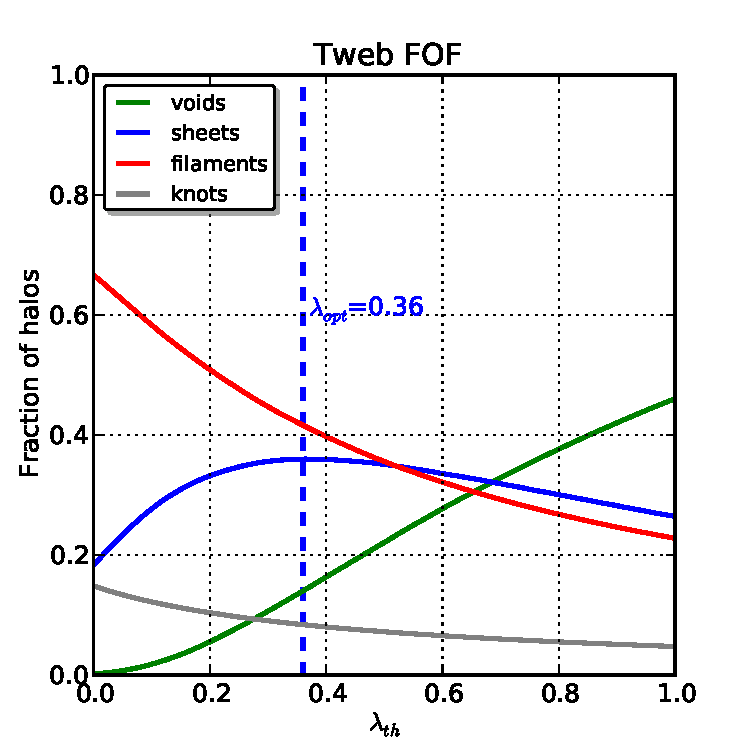
\includegraphics[trim = 0mm 0mm 5mm 5mm, clip, keepaspectratio=true,
  width=0.25\textheight]{./figures/halos_fraction_FOF_Tweb.pdf}
  
  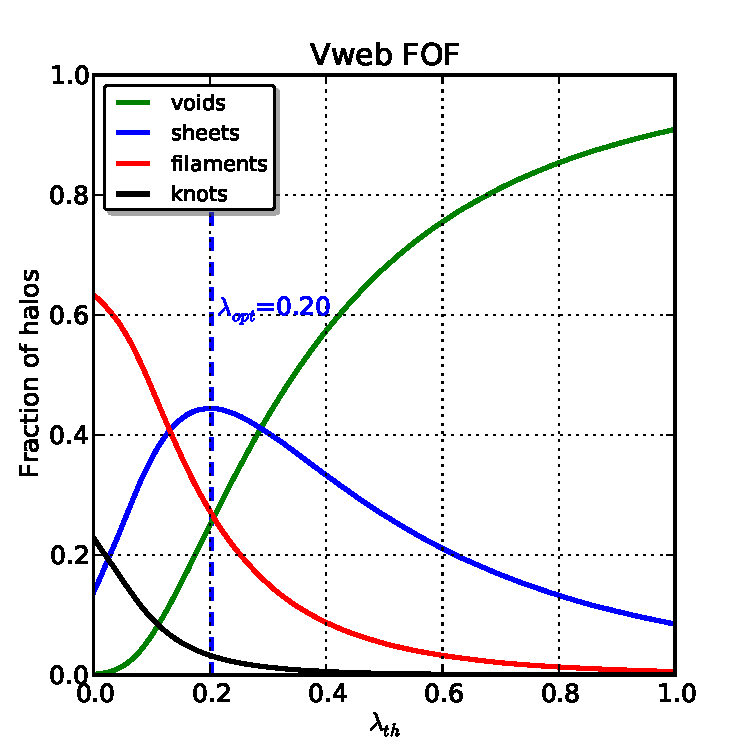
\includegraphics[trim = 0mm 0mm 5mm 5mm, clip, keepaspectratio=true,
  width=0.25\textheight]{./figures/halos_fraction_FOF_Vweb.pdf}

  \captionof{figure}{\small Mean density parameter for each one of the 
  defined environments according to the chosen $\lambda_{th}$ value and 
  for both classification schemes. Tweb (green lines) and Vweb (blue 
  lines). The mean density parameter is calculated by averaging all the 
  values  of the cells determined as a certain type of environment 
  according to its eigenvalues. The optimal parameters found are 
  $\lambda_{opt}^{T}=0.326$ and $\lambda_{opt}^{V}=0.188$.}

  \label{fig:halos_fractions}
  \vspace{0.1 cm}

\end{figure}
\end{flushleft}
%.........................................................................



%.........................................................................
%FIGURE 2: Visual impression of the cosmic web
\begin{flushleft}
\begin{figure*}
\centering

  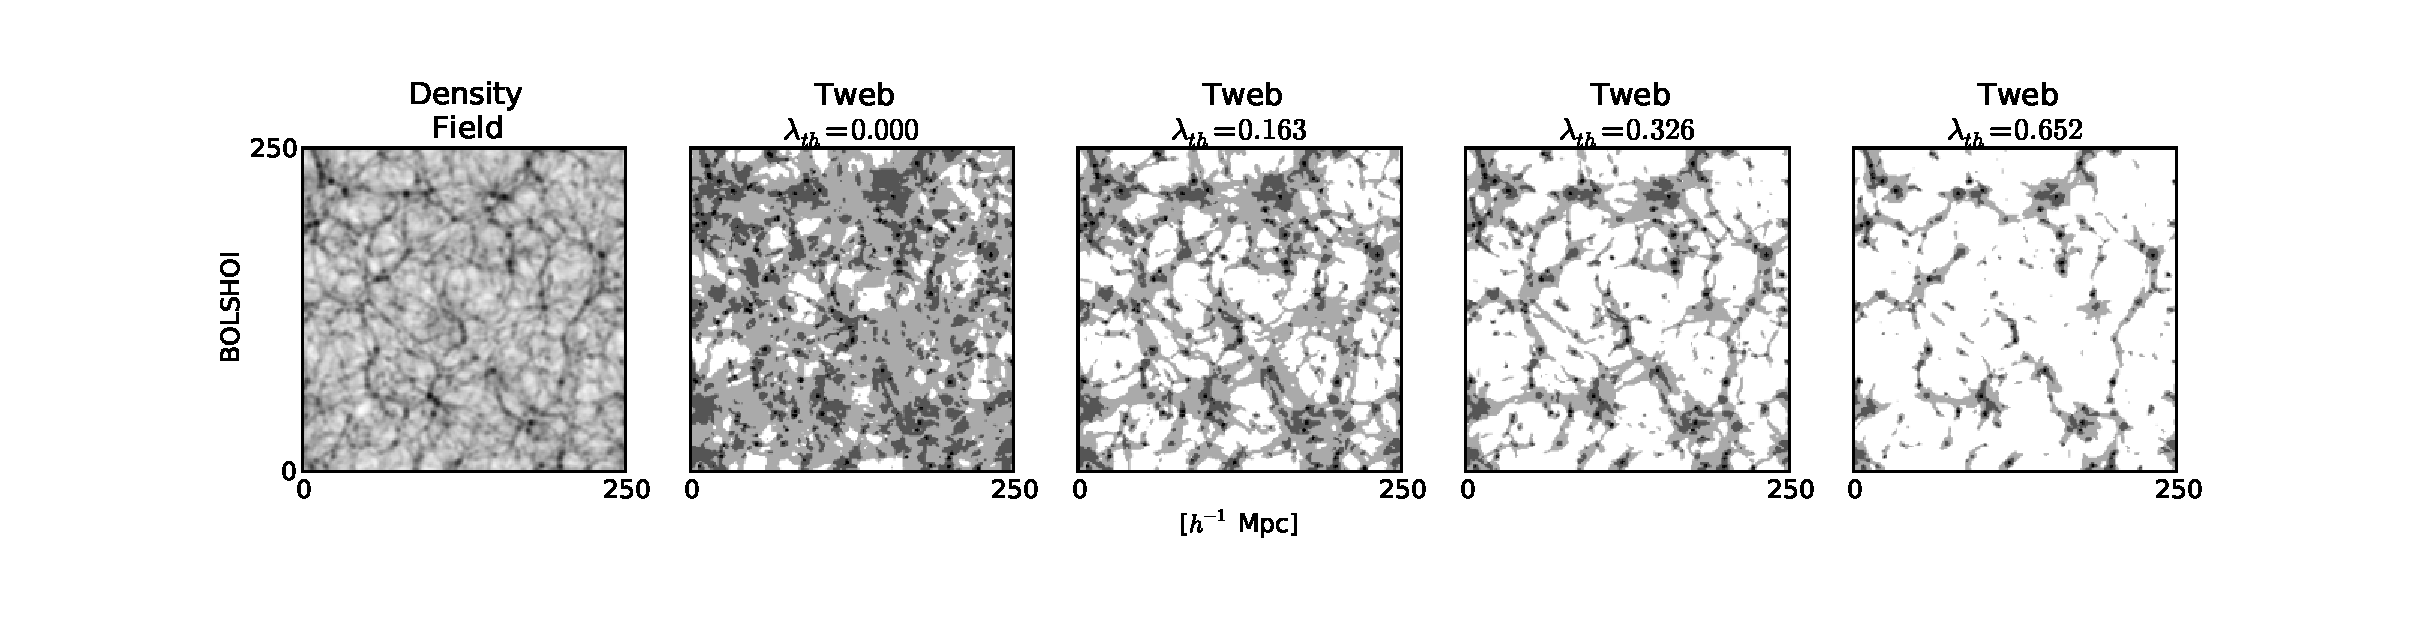
\includegraphics[trim = 42mm 15mm 37mm 10mm, clip, keepaspectratio=true,
  width=0.75\textheight]{./figures/cosmicweb_visual_Tweb.pdf}
  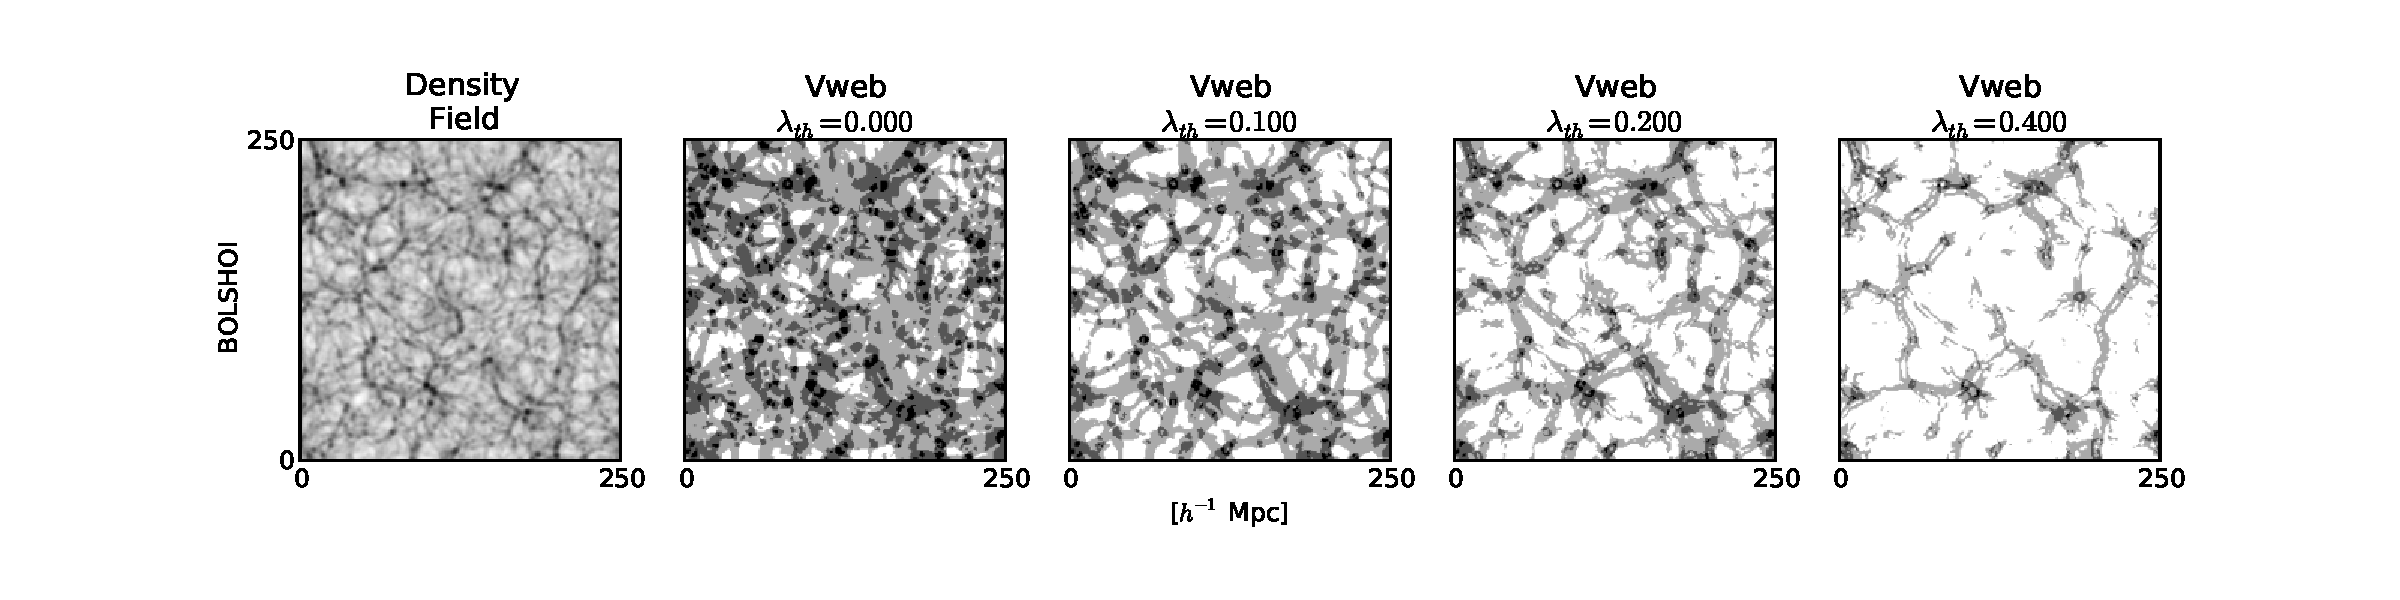
\includegraphics[trim = 42mm 15mm 37mm 10mm, clip, keepaspectratio=true,
  width=0.75\textheight]{./figures/cosmicweb_visual_Vweb.pdf}
  
  \captionof{figure}{\small Visual impression of the density field (left 
  panels), and of each classification scheme with the $\lambda_{th}$ values 
  obtained by our criteria (others panels). The color convention for each 
  environment is (white) - void, (light gray) - sheet, (gray) - filament, 
  (black) - knot. For each web scheme, it has been used the previously 
  established optimal threshold as a reference value, so plots are done 
  with the next values $\lambda_{th} = 0.0$, $\lambda_{th} = 
  \lambda_{opt}/2$, $\lambda_{th} = \lambda_{opt}$ and $\lambda_{th} = 
  2\lambda_{opt}$.}

  \label{fig:visual_impression}
  \vspace{0.1 cm}

\end{figure*}
\end{flushleft}
%.........................................................................


\end{document}
